\documentclass[a4paper,14pt]{extreport}
  \usepackage[left=1.5cm,right=1.5cm,
      top=1.5cm,bottom=2cm,bindingoffset=0cm]{geometry}
  \usepackage{scrextend}
  \usepackage[T1,T2A]{fontenc}
  \usepackage[utf8]{inputenc}
  \usepackage[english,russian,ukrainian]{babel}
  \usepackage{tabularx}
  \linespread{1.3}
  \usepackage{amssymb}
  \usepackage{color}
  \usepackage{amsmath}
  \usepackage{mathrsfs}
  \usepackage{listings}
  \usepackage{graphicx}
  \graphicspath{ {./images/} }
  \usepackage{lipsum}
  \usepackage{xcolor}
  \usepackage{hyperref}
  \usepackage{tcolorbox}
  \usepackage{tikz}
  \usepackage[framemethod=TikZ]{mdframed}
  \usepackage{wrapfig,boxedminipage,lipsum}
  \mdfdefinestyle{MyFrame}{%
  linecolor=blue,outerlinewidth=2pt,roundcorner=20pt,innertopmargin=\baselineskip,innerbottommargin=\baselineskip,innerrightmargin=20pt,innerleftmargin=20pt,backgroundcolor=gray!50!white}
   \usepackage{csvsimple}
   \usepackage{supertabular}
  \usepackage{pdflscape}
  \usepackage{fancyvrb}
  %\usepackage{comment}
  \usepackage{array,tabularx}
  \usepackage{colortbl}

  \usepackage{varwidth}
  \tcbuselibrary{skins}
  \usepackage{fancybox}
  \usepackage{spreadtab}


  \usepackage{tikz}
  \usepackage[framemethod=TikZ]{mdframed}
  \usepackage{xcolor}
  \usetikzlibrary{calc}
  \makeatletter
  \newlength{\mylength}
  \xdef\CircleFactor{1.1}
  \setlength\mylength{\dimexpr\f@size pt}
  \newsavebox{\mybox}
  \newcommand*\circled[2][draw=blue]{\savebox\mybox{\vbox{\vphantom{WL1/}#1}}\setlength\mylength{\dimexpr\CircleFactor\dimexpr\ht\mybox+\dp\mybox\relax\relax}\tikzset{mystyle/.style={circle,#1,minimum height={\mylength}}}
  \tikz[baseline=(char.base)]
  \node[mystyle] (char) {#2};}
  \makeatother
   % Цвета для гиперссылок
  \definecolor{linkcolor}{rgb}{0, 0.72, 0.92} % цвет ссылок
  \definecolor{urlcolor}{rgb}{0.0, 0.0, 1.0}% цвет гиперссылок
  \hypersetup{pdfstartview=FitH,  linkcolor=linkcolor,urlcolor=urlcolor,citecolor=red, colorlinks=true}

  \definecolor{ggreen}{rgb}{0.4,1,0}
  \definecolor{rred}{rgb}{1,0.1,0.1}
  \definecolor{amber}{rgb}{1.0, 0.75, 0.0}
  \definecolor{babyblue}{rgb}{0.54, 0.81, 0.94}
  \definecolor{amethyst}{rgb}{0.6, 0.4, 0.8}

  \usepackage{float}
  \usepackage{wrapfig}
  \usepackage{framed}
  %for nice Code{
  \lstdefinestyle{customc}{
    belowcaptionskip=1\baselineskip,
    breaklines=true,
    frame=L,
    xleftmargin=\parindent,
    language=C,
    showstringspaces=false,
    basicstyle=\small\ttfamily,
    keywordstyle=\bfseries\color{green!40!black},
    commentstyle=\itshape\color{purple!40!black},
    identifierstyle=\color{blue},
    stringstyle=\color{orange},
  }
  \lstset{escapechar=@,style=customc}
%}


\begin{document}
%------------------------------1
  \noindent{\color{blue} \rule{\linewidth}{0.7mm}}
  \begin{center}1\end{center}
  \noindent{\color{blue} \rule{\linewidth}{0.7mm}}

  Перший апарат магнітного запису винайшов і побудував датський інженер Вальдемар Поульсен. Апарат назвали телеграфоном і призначався він для зберігання звуку. Телеграфон був запатентований в 1898 році, і цю дату вважають роком народження магнітного запису.\par
  \begin{figure}[h]
  \center{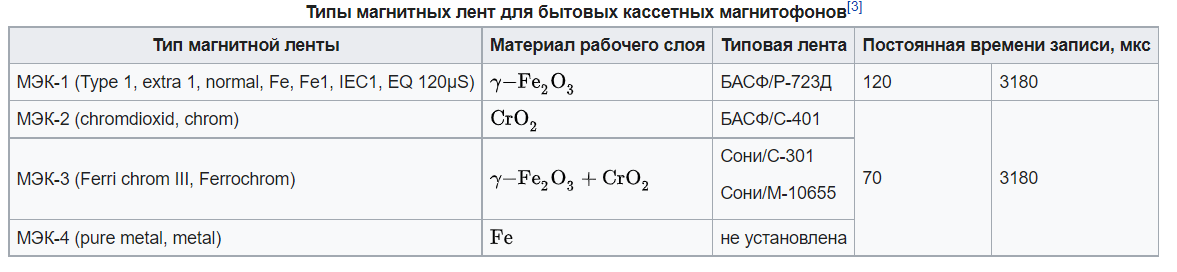
\includegraphics[width=0.9\linewidth]{forp1.png}}
  \end{figure}
  Поульсен створив кілька різновидів апаратів для магнітного запису. В одному з них дріт (носій запису) намотаний на немагнітний валик, який утворює на ньому магнітний робочий шар у вигляді циліндричної спіралі. В процесі запису або відтворення валик разом з дротом
  обертався відносно магнітної головки, яка переміщалася паралельно його осі, ковзаючи по виткам дроту, як по різьбі гвинта. В ролі магнітної головки використовувався електромагніт, що складався з стрижневого осердя, який одним кінцем ковзав по носію, і котушки мідного дроту. Головка з сердечником створювала досить сильне і сконцентроване магнітне поле, за допомогою якого можна було записувати звукові частоти.\par
%------------------------------2
\noindent{\color{blue} \rule{\linewidth}{0.7mm}}
\begin{center}2\end{center}
\noindent{\color{blue} \rule{\linewidth}{0.7mm}}

%------------------------------3
  \noindent{\color{blue} \rule{\linewidth}{0.7mm}}
  \begin{center}3\end{center}
  \noindent{\color{blue} \rule{\linewidth}{0.7mm}}
  Основа магнітної стрічки виготовляється з синтетичних матеріалів, найчастіше ацетатцелюлозних (діацетату і триацетату), поліетилентерефталату (лавсану) і полиимидов. Застосовувалися й інші матеріали (папір, целулоїд, поліетилен, поліхлорвініл), але вони вийшли з ужитку, так як гірше відповідали вимогам, що пред'являються до магнітних стрічок.\\

  В якості робочого шару використовуються порошки оксидів заліза, хрому, кобальту і їх суміші, а також порошки чистих металів. Від складу, товщини і однорідності робочого шару, розмірів і форми частинок магнітного порошку в чому залежать основні характеристики стрічки.

%------------------------------4
  \noindent{\color{blue} \rule{\linewidth}{0.7mm}}
  \begin{center}4\end{center}
  \noindent{\color{blue} \rule{\linewidth}{0.7mm}}
  Фізично технологія запису на жорсткі диски і плівки одна і та ж: дані записуються на намагнічену поверхню вузькими доріжками, на яких відбувається перемикання полярності. Інформація записується послідовністю бітів.\\
  За останнє десятиліття плівка розвивалася не менш, ніж жорсткі диски або транзистори. Перша плівка для зберігання інформації в цифровому вигляді - модель 726 виробництва IBM - могла зберігати 1,1 МБ на котушці. Сьогодні 1 котушка здатна зберігати 15 терабайт даних, а одне роботизоване плівкове сховище - 278 петабайт.\\ 

  Щоб домогтися такого прогресу, інженери пристосували головки для читання і запису рухатися по вкрай вузьких доріжках на плівці - близько 100 нанометрів шириною. Крім цього, довелося зробити зчитувальні головки вужчими - близько 50 нанометрів шириною. При зчитуванні рівень сигналу до шуму теж зменшився, тому довелося маніпулювати розміром і положенням намагнічених гранул і гладкістю поверхні плівки, а також удосконалити процес обробки сигналу і помилок зчитування.\par

%------------------------------5
  \noindent{\color{blue} \rule{\linewidth}{0.7mm}}
  \begin{center}5\end{center}
  \noindent{\color{blue} \rule{\linewidth}{0.7mm}}
  Як вже було описано раніше, магнітний запис інформації заснована на тому, що багато матеріалів в магнітному полі намагнічуються вздовж його ліній і зберігають цю намагніченість навіть після відключення поля. У магнітних носіях, таких як дискети і HDD, роль бітів виконує намагніченість невеликих ділянок диска. Зі зменшенням розмірів цих ділянок значно зростає обсяг інформації, яку можна записати на пристрої того ж розміру. Зараз один домен комерційно доступних жорстких дисків налічує в собі близько мільйона атомів (кілька нанометрів в діаметрі). Експерименти показують, що розмір комірки можна зменшити до 3-12 атомів.\par

  Автори нової роботи домоглися стабільного запису і зберігання інформації протягом декількох годин в одиночних атомах гольмію. Вибір металу вчені пояснюють наступним чином. Будь-яка орбіталь атома може нести на собі жодного, один або два електрони. Магнітні властивості атомів визначаються в основному неспареними електронами, які знаходяться на своїй орбіталі на самоті. Гольмій володіє великою кількістю неспарених електронів і, до того ж, є має найбільший магнітний момент серед елементів періодичної таблиці. Крім того, неспарені електрони атома знаходяться близько до ядра, що забезпечує їх деяку ізольованість від зовнішнього середовища. Тому магнітний стан гольмію може зберігатися досить довгий час.\par

  На поверхні оксиду магнію Гольмій відчуває магнітну анізотропію - вона призводить до того, що у атома є два стійких магнітних стана, що визначаються орієнтацією його сумарного спіна. Щоб перейти з одного стану в інший атом повинен подолати енергетичний бар'єр. Чим нижче температура середовища, тим менш імовірний цей перехід. Відповідно цим двох стійким станам і приписуються значення «нуля» і «одиниці».\par

%------------------------------6
  В експерименті вчені створили комірку пам'яті, що складалася з двох атомів гольмію, що знаходяться на поверхні оксиду магнію, який був охолоджений до 1,2 Кельвіна. Для запису і читання вчені використовували скануючий тунельний мікроскоп, який досліджує поверхні за допомогою надзвичайно гострої голки. Операція запису полягала в додаванні до атому певної електричної напруги. Для читання автори використовували ефект тунельного магнітоопору - електричний опір між поверхнею і голкою залежить від напрямків намагніченості кінчика голки і атома гольмію. \par

%------------------------------7
....

%------------------------------8














































\end{document}